\subsubsection{ミュータブルなリスト構造}
ペアに対する操作 (\lstinline{cons}, \lstinline{car}, \lstinline{cdr})は
リストを作る, リストから要素を取り出すために使うことができるが, その操作を用いて
リストを変えることができない. \lstinline{append}や\lstinline{list}も
以上の操作で定義されているので, 同じことが言える. リストを変えるために新しい
操作が必要となる.

ペアに対して基本的なミュテータは\lstinline{set-car!}と\lstinline{set-cdr!}である.
使い方の例を以下に示す.

\begin{lstlisting}[basicstyle=\footnotesize]
(define foo (cons 1 2))
(set-car! foo 2)
(set-cdr! foo 3)
foo => (2 3)
\end{lstlisting}

その2つのミューテータを用いてリストを変えることができる. 例えば,
\begin{lstlisting}[basicstyle=\footnotesize]
(define x '((a b) c d))
(define y '(e f))
\end{lstlisting}
のようなリストが定義されているとすると,
\begin{lstlisting}[basicstyle=\footnotesize,caption=]
(set-car! x y)
\end{lstlisting}
を行うと, 元々\lstinline{(a b)}だった\lstinline{(car x)}が\lstinline{(e f)}に
なる.
その実行のプロセスは図\ref{fig:base-list}と\ref{fig:changed-list}で
図として表す.

\begin{figure}[t]
  \begin{minipage}{0.48\linewidth}
    \centering
    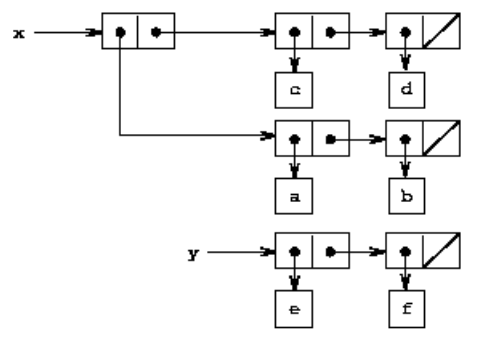
\includegraphics[height=5cm,width=6cm]{imgs/base_list.png}
    \caption{\label{fig:base-list}x: ((a b) c d), y: (e f)}
  \end{minipage}
  %
  \begin{minipage}{0.48\linewidth}
    \centering
    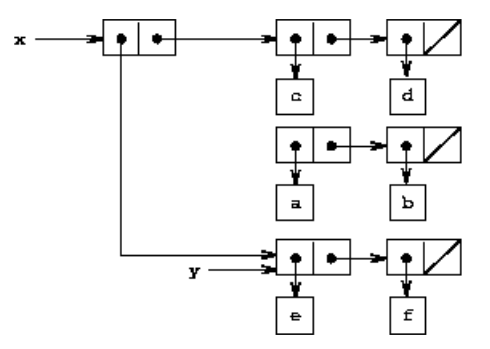
\includegraphics[height=5cm,width=6cm]{imgs/changed_list.png}
    \caption{\label{fig:changed-list}(set-car! x y)の効果}
  \end{minipage}
\end{figure}

\lstinline{set-cdr!}は\lstinline{set-car!}と同じような仕様と効果であるが,
ペアの1つ目の要素ではなく, 2つ目の要素に適用される.

\paragraph{データ構造の共有} ペアが複数のデータ構造で共有される可能性もある.
次の例について考える.

\begin{lstlisting}[basicstyle=\footnotesize,caption=]
(define x '(a b))
(define z1 (cons x x))
\end{lstlisting}

と定義した時に, \lstinline{(car z1)}も\lstinline{(cdr z1)}も
同じく\lstinline{x}となっているので, \lstinline{(set-car! x 'c)}
を実行したら, \lstinline{(car z1)}も\lstinline{(cdr z1)}も\lstinline{(c b)}に
なってしまう. それに対して,

\begin{lstlisting}[basicstyle=\footnotesize,caption=]
(define z2 (cons '(a b) '(a b)))
\end{lstlisting}

と定義したら, \lstinline{(car z2)}と\lstinline{(cdr z2)}は別のデータを
指すので, \lstinline{(set-car! (car z2) 'x)}を実行すると, \lstinline{(car z2)}が
\lstinline{(y b)}になるが, \lstinline{(cdr z2)}は\lstinline{(a b)}のままになる.
その仕様を図で表す.

\begin{figure}[b]
  \begin{minipage}{0.48\linewidth}
    \centering
    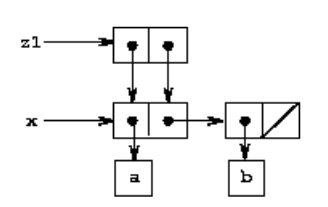
\includegraphics[height=3cm,width=6cm]{imgs/shared_pair.png}
    \caption{\label{fig:shared-pair}共有されているデータオブジェクト}
  \end{minipage}
  %
  \begin{minipage}{0.48\linewidth}
    \centering
    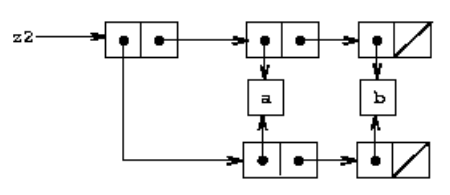
\includegraphics[height=3cm,width=6cm]{imgs/not_shared_pair.png}
    \caption{\label{fig:not-shared-pair}共有されていないデータオブジェクト}
  \end{minipage}
\end{figure}